\documentclass[10pt]{beamer}

\usetheme{CambridgeUS}
\usepackage[english, russian]{babel}
\usepackage[utf8]{inputenc}
\usepackage{caption}
\usepackage{etoolbox}
\usepackage{multicol}
\usepackage{listings}
\usepackage{wasysym}
\usepackage{mathtools}
\DeclarePairedDelimiter\ceil{\lceil}{\rceil}
\DeclarePairedDelimiter\floor{\lfloor}{\rfloor}

\definecolor{mygreen}{rgb}{0,0.6,0}
\lstset{
  basicstyle=\ttfamily\footnotesize,        % the size of the fonts that are used for the code
  breaklines=true,                 % automatic line breaking only at whitespace
  captionpos=b,                    % sets the caption-position to bottom
  commentstyle=\color{mygreen},    % comment style
  keywordstyle=\color{blue},       % keyword style
  stringstyle=\color{red},     % string literal style
  showstringspaces=false,
  morekeywords={include, printf},
  texcl=true     %<---- added
}


\title[\href{https://goo.gl/NRgp8K}{https://goo.gl/NRgp8K} (Term 1)]{Базовые АТД и структуры данных}
\author[Гусев Илья, Булгаков Илья]{Гусев Илья, Булгаков Илья}
\institute[МФТИ] 
{Московский физико-технический институт\\*}
\date{Москва, 2018}
\subject{Computer Science}

\begin{document}

\begin{frame}
  \titlepage
\end{frame}

\begin{frame}{Содержание}
\tableofcontents
\end{frame}

\section{АТД vs структуры данных}
\begin{frame}[fragile]{АТД vs структуры данных}
АТД - абстрактный тип данных.\\
Набор функций, независимых от конкретной реализации типа, для оперирования его значениями.\\
Реализация скрыта, по сути представляет из себя интерфейс. \\
В С++ это абстрактный класс, все функции которого чисто виртуальны (pure virtual). \\
\end{frame}

\begin{frame}[fragile]{АТД vs структуры данных}{Примеры}
\begin{itemize}
    \item Стек (push\_back, pop\_back)
        \begin{enumerate}
            \item Реализация динамическим массивом
            \item Реализация связным списком
        \end{enumerate}
    \item Очередь (push\_back, pop\_front)
        \begin{enumerate}
            \item Реализация динамическим массивом
            \item Реализация связным списком
            \item Реализация двумя стеками
        \end{enumerate}
    \item Очередь с приоритетами (insert(ключ, значение), extract\_minimum $\rightarrow$ (ключ, значение))
        \begin{enumerate}
            \item Реализация динамическим массивом
            \item Реализация связным списком
            \item Реализация двоичной кучей
            \item Реализация биномиальной кучей
            \item Реализация фибоначчиевой кучей
        \end{enumerate}
\end{itemize}
\end{frame}

\begin{frame}[fragile]{АТД vs структуры данных}{Подробнее про стек и очередь}
External/stacks-algs4.cs.princeton.edu.pdf
\end{frame}

\section{Структуры данных}
\subsection{Куча}
\begin{frame}[fragile]{Двоичная куча (heap)}
\begin{multicols}{2}
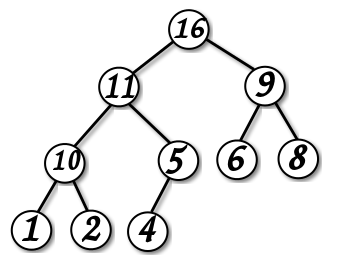
\includegraphics[width=5cm, height=4cm]{Term_1/Source/Pirctures/max-heap2.png}
\vfill\eject
\begin{enumerate}
    \item Двоичное дерево (связный ациклический граф, у которого у любой вершины не больше 2 потомков)
    \item Если узел B являетсeя потомком узла A, то $A.key \geq B.key$ (max-куча). Для min-кучи наоборот.
    \item Глубина всех листьев (расстояние до корня) отличается не более чем на 1 слой.
    \item Последний слой заполняется слева направо без «дырок».
\end{enumerate}
\end{multicols}
\end{frame}

\begin{frame}[fragile]{Двоичная куча (heap, пирамида)}{Реализация}
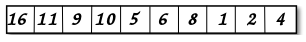
\includegraphics[width=10cm, height=1.5cm]{Term_1/Source/Pirctures/max-heap-array.png}\\
\begin{itemize}
    \item $A[0]$ - корень\\
    \item $\forall i$ $A[2i+1]$ - левый потомок $A[i]$\\
    \item $\forall i$ $A[2i+2]$ - правый потомок $A[i]$
\end{itemize}
\end{frame}

\begin{frame}[fragile]{Двоичная куча (heap, пирамида)}{Действия и сложность}
\begin{itemize}
    \item Добавить элемент в кучу. Сложность $\mathcal{O}(\log {n})$
    \item Исключить максимальный элемент из кучи. Время работы  $\mathcal{O}(\log {n})$
    \item Изменить значение любого элемента. Время работы  $\mathcal{O}(\log {n})$
    \item Превратить неупорядоченный массив элементов в кучу. Сложность  $\mathcal{O}(n)$ 
    
\includegraphics[height=3em]{Term_1/Source/Pirctures/thinking-emoji-circle.jpeg}
    
\includegraphics[height=3em]{Term_1/Source/Pirctures/thinking-emoji-big.png}
    
\includegraphics[height=3em]{Term_1/Source/Pirctures/thinking-emoji-paint.png}
\end{itemize}
\end{frame}

\begin{frame}[fragile]{Двоичная куча (heap, пирамида)}{Построение за $\mathcal{O}(n)$ }
$\ceil{\frac{n}{2^{h+1}}}$ - максимум количества элементов на уровне h\\
$\mathcal{O}(h)$ - сложность вставки элемента на уровень h\\
$\floor{\lg(n)}$ - высота n-элементной пирамиды\\
$$\sum_{h=0}^{\floor{\lg(n)}} \ceil{\frac{n}{2^{h+1}}} \mathcal{O}(h) = \mathcal{O}(n \sum_{h=0}^{\floor{\lg(n)}} \frac{h}{2^h}) $$
$$ \sum_{h=0}^{\infty} \frac{h}{2^h} = \frac{1/2}{(1-1/2)^2} = 2$$
$$ \mathcal{O}(n \sum_{h=0}^{\floor{\lg(n)}} \frac{h}{2^h}) = \mathcal{O}(n \sum_{h=0}^{\infty} \frac{h}{2^h}) = \mathcal{O}(2n) =  \mathcal{O}(n)$$
\end{frame}

\begin{frame}[fragile]{Двоичная куча (heap, пирамида)}{Вставка и extract\_min}
\begin{multicols}{2}
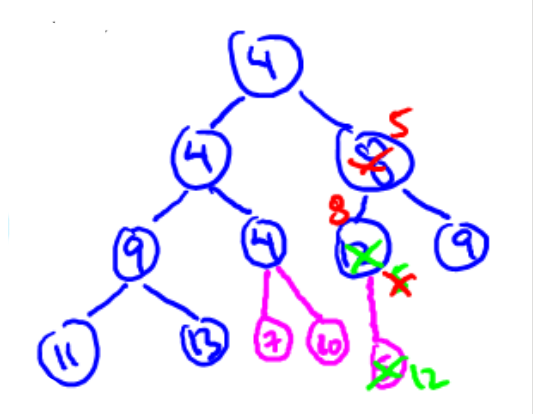
\includegraphics[width=5cm, height=4cm]{Term_1/Source/Pirctures/bubble-up.png}
\vfill\eject
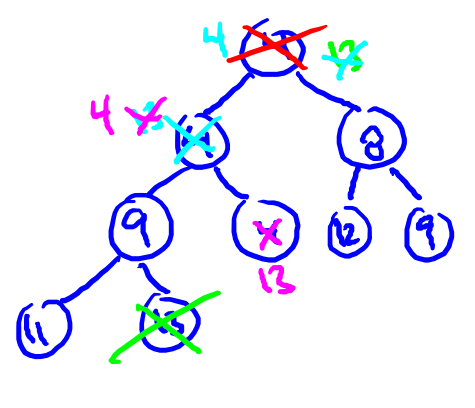
\includegraphics[width=5cm, height=4cm]{Term_1/Source/Pirctures/bubble-down.png}
\end{multicols}
\end{frame}

\appendix
\section<presentation>*{\appendixname}
\subsection<presentation>*{Useful links}

\begin{frame}[allowframebreaks]
  \frametitle<presentation>{Полезные ссылки}
    
  \begin{thebibliography}{10}
{
  \beamertemplatearticlebibitems
  
  \bibitem{Kormen1}
  \texttt{Т.Кормен, Ч.Лейзерсон, Р.Ривест, К.Штайн - Алгоритмы. Построение и анализ. Глава 6}
  \newblock \href{https://bit.ly/2wFzphU}{\texttt{https://bit.ly/2wFzphU}}
  
  \bibitem{prineston}
  \texttt{Lecture Slides for Algorithm Design}
  \newblock \href{https://algs4.cs.princeton.edu/lectures/}{\texttt{https://algs4.cs.princeton.edu/lectures/}}

}


  \end{thebibliography}
\end{frame}

\end{document}


